\documentclass[12pt]{article}

%% Language and font encodings
\usepackage[spanish]{babel}
\usepackage[utf8x]{inputenc}
\usepackage[T1]{fontenc}

%% Sets page size and margins
\usepackage[a4paper,top=3cm,bottom=2cm,left=3cm,right=3cm,marginparwidth=1.75cm]{geometry}
\linespread{1.5}

%% Useful packages
\usepackage{amsmath}
\usepackage{amssymb}
\usepackage{graphicx}
\usepackage[colorinlistoftodos]{todonotes}
\usepackage[colorlinks=true, allcolors=blue]{hyperref}
\usepackage{float}

\title{Efecto de Aharonov-Bohm}
\author{Siria Sadeddin , 08-11245}

\begin{document}
\maketitle

\begin{abstract}
El efecto de Aharonov-Bohm es un fenómeno mecánico cuántico en el cual una partícula  cargada es afectada por un potencial electromagnético cuando esta se encuentra en una región donde \textbf{B} y \textbf{E} son cero. 
\end{abstract}
\section{Introducción}
De acuerdo con la Mecánica Cuántica, el movimiento de una partícula cargada puede ser influenciado por la presencia de campos electromagnéticos en regiones donde la partícula se encuentra excluida del campo. Este fenomeno es llamado el efecto \textit{Aharonov-Bohm} (efecto AB). Después de la publicación del articulo "Significance of Electromagnetic
Potentials in the Quantum Theory, by Y. Aharonov and D. Bohm (1959)"  muchas publicaciones se han hecho en torno a lo que el efecto AB nos enseña sobre la influencia de los campos electromagnéticos en partículas cargadas, esto suponiendo que la Mecánica Cuántica describe de manera correcta la naturaleza. \\
Sin embargo muchos científicos se han mostrado escépticos ante la idea de que una partícula pueda ser dispersada en regiones donde la partícula está excluida del campo. Ante esto se ha invocado el \textit{Teorema de Erhenfest} para probar que el efecto AB es un error de cálculo. \\
Cientos de artículos se han publicado desde la primera publicación de Aharonov y Bohm. Se han hecho modificaciones a la Mecánica Cuántica de manera que esta no exhibe el efecto AB, pero han fallado al ser contrastadas con otras predicciones de la Mecánica Cuántica. También se han hecho cálculos clásicos suponiendo que la dispersión de la partícula se debe a la interacción clásica de ésta con la fuente del campo, y no con el campo en sí en la región excluida de este.\\
Sin embargo todas estas ideas han sido refutadas por análisis teóricos que comprueban las conclusiones y a veces las interpretaciones de Aharonov y Bohm.\\
\begin{figure}
\centering
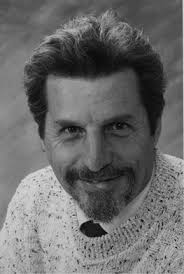
\includegraphics[scale=.6]{img/aharonov.jpg}
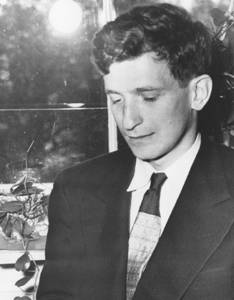
\includegraphics[scale=.7]{img/bohm.jpg}
\caption{Yakir Aharonov (1932-) a la izquierda,  es un físico israelí especializado en Física Cuántica y tiene una cátedra en la Universidad de Tel Aviv en Israel y la Universidad de Carolina del Sur en los Estados Unidos desde 1973. David Joseph Bohm (1917-1992) a la derecha, fue un físico estadounidense que hizo importantes contribuciones en los campos de la física teórica, la epistemología y la neuropsicología}
\end{figure}

Experimentos de interferencia de electrones se han llevado a cabo para una confirmación directa del efecto, cada vez estos se hacen con mayor precisión y mejor aislamiento de campos externos, ya que los detractores del efecto AB argumentan que la dispersión de los electrones se debe a la influencia de campos externos que afectan el experimento; pero esto ha sido superado por las conclusiones experimentales.\\
 Werner Ehrenberg (1901–1975) y Raymond E. Siday fueron los primeros en predecir el fenómeno en 1949.  Yakir Aharonov y David Bohm fueron los primeros en publicar sobre el efecto por separado en 1959. En los siglos XVIII y XIX la física estaba dominada por la dinámica newtoniana. El fenómeno electromagnético podía ser descrito a través del movimiento de cargas como consecuencia de los campos que actúan sobre ellas. En este modelo, los campos pueden definirse de forma única (gracias a las ecuaciones de Maxwell), más los potenciales no, por lo que estos últimos eran considerados como simples objetos matemáticos. El fenómeno electromagnético puede ser descrito en términos de un potencial escalar $\phi$ y un potencial vectorial $\vec{A}$. El efecto Aharonov-Bhom demostró que incluso en regiones donde los campos electromagnéticos se anulan, las partículas son afectadas por el potencial electromagnético. \\
 Con el desarrollo de la Mecánica Cuántica a principios de los años 20, el enfoque clásico de la teoría electromagnética se vio cuestionado, ya que en la ecuación de Shrodinger para sistemas en presencia de campos electromagnéticos no aparecen los campos, sino potenciales (es decir, el estado de una partícula cuántica puede ser descrito a partir de los potenciales electromagnéticos). 

\section{Algo de Teoría}

\subsection{Enfoque clásico}

Antes de adentrarnos en la teoría electromagnética cuántica, recordemos algo de teoría electromagnética clásica.\\
En 1861, el físico y matemático escoces James Clerk Maxwell escribió las cuatro ecuaciones diferenciales que son la base de la teoría electromagnética.

\begin{equation}
\nabla\cdot\vec{E}=\rho/\epsilon_o
\end{equation}
\begin{equation}
\nabla\cdot\vec{B}=0
\end{equation}
\begin{equation}
\nabla\times\vec{E}=-\frac{\partial\vec{B}}{\partial t}
\end{equation}
\begin{equation}
\nabla\times\vec{B}=\mu_o\vec{j}+\mu_o\epsilon_o\frac{\partial\vec{E}}{\partial t}
\end{equation}



Las ecuaciones de Maxwell junto con la fuerza de Lorentz 
$\vec{F}=e(\vec{E}+\vec{v\times\vec{B}})$ describen la mayor parte de la física electromagnética clásica. \\
De las ecuaciones observamos que $\vec{B}$ tiene divergencia nula, por lo que podemos escribirlo como: 

\begin{equation}
\vec{B}=\nabla\times\vec{A}
\end{equation}


Donde $\vec{A}$ es el potencial vectorial. De manera similar se puede mostrar que:
\begin{equation}
\vec{E}=-\nabla\phi-\frac{\partial\vec{A}}{\partial t}
\end{equation}

Donde $\phi$ es el potencial escalar.\\
Los potenciales escalar y vectorial pueden transformarse de la manera siguiente sin afectar los campos $\vec{B}$ y $\vec{E}$ resultantes.

\begin{equation}
\vec{A'}=\vec{A}+\nabla\chi
\end{equation}

\begin{equation}
\phi'=\phi-\frac{\partial \chi }{\partial t}
\end{equation}



Es decir, $\vec{B}$ y $\vec{E}$ son invariantes bajo estas transformaciones de $\vec{A}$ y $\phi$. Estas transformaciones llevan el nombre de "Transformaciones de Gauge", y debido la invarianza de las ecuaciones de Maxwell bajo ellas. Por mucho tiempo se pensó que los potenciales $\vec{A}$ y $\phi$ eran solo un constructo matemático sin significado físico. 
\subsubsection{\textbf{Demostracion de la invarianza de las transformaciones de Gauge en las ecuaciones de Maxwell:}}


\begin{equation}
B'=\nabla\times\vec{A'}=\nabla\times\vec{A}
\end{equation}

\begin{equation}
\begin{split}
\nabla\times(\vec{A}+\nabla\chi) &=\nabla\times\vec{A}+\nabla\times(\nabla\chi)\\ & =\nabla\times\vec{A}
\end{split}
\end{equation}

\begin{equation}
\implies B'=\nabla\times\vec{A}
\end{equation}

\begin{equation}
\therefore B'=B
\end{equation}

\begin{equation}
\begin{split}
E'& =-\nabla\phi'-\frac{\partial\vec{A'}}{\partial t}\\
& =-\nabla(\phi-\frac{\partial\chi}{\partial t})-\frac{\partial(\vec{A}+\nabla\chi)}{\partial t} \\ 
&  =-\nabla\phi+\nabla\frac{\partial\chi}{\partial t}-\frac{\partial(\vec{A})}{\partial t}-\frac{\partial\nabla\chi}{\partial t}
\end{split}
\end{equation}


\begin{equation}
\frac{\partial\nabla\chi}{\partial t}=\frac{\nabla\partial\chi}{\partial t}
\end{equation}

\begin{equation}
\implies E'=-\nabla\phi-\frac{\partial\vec{A}}{\partial t}=E
\end{equation}

\begin{equation}
\therefore  E'=E
\end{equation}

\subsection{Enfoque cuántico}
En mecánica cuántica, la dinámica de una partícula esta determinada por la ecuación de Shrodinger

\begin{equation}
H\Psi=i\hbar\frac{\partial\Psi}{\partial t}
\end{equation}


Donde H es el operador de Hamilton que en el caso de una partícula cargada en un campo electromagnético esta dado por
\begin{equation}
H=\frac{1}{2m}(i\hbar\nabla+e\vec{A}(\vec{r}))^2+e\phi(\vec{r})+V(\vec{r})
\end{equation}


Donde $V(\vec{r})$ representa un potencial no eléctrico.
El operador de Hamilton es invariante ante las transformaciones de Gauge.\\

\subsubsection{\textbf{Demostración de la invarianza del operador de Hamilton ante las transformaciones de Gauge}}
\begin{equation}
(H'-i\hbar\frac{\partial}{\partial t})|\Psi\rangle=0
\end{equation}
\begin{equation}
H'=\frac{1}{2m}(i\hbar\nabla+e\vec{A'}(\vec{r}))^2+e\phi'(\vec{r})+V(\vec{r})
\end{equation}

Sabemos que 
\begin{equation}
i\hbar\nabla+e\vec{A'}(\vec{r})=i\hbar\nabla+e(\vec{A}+\nabla\chi)
\end{equation}

Introducimos un operador $U=e^{ie\chi/\hbar}$  unitario ($UU^{\dag}$=I), tal que : 

\begin{equation}
|\Psi'\rangle=U|\Psi\rangle
\end{equation}
Apliquemos la transformación a $H$ para esto primero evaluemos que le pasa a $i\hbar\nabla+e\vec{A'}(\vec{r})$ ante la transformación
\begin{equation}
\begin{split}
(U(i\hbar\nabla+e\vec{A}(\vec{r}))U^{\dag})|f\rangle &=
(e^{ie\chi/\hbar}(i\hbar\nabla+e\vec{A}(\vec{r}))e^{-ie\chi/\hbar})|f\rangle \\
&=e^{ie\chi/\hbar}i\hbar\nabla(e^{-ie\chi/\hbar}|f\rangle)+e^{ie\chi/\hbar}e\vec{A}(\vec{r})e^{-ie\chi/\hbar}|f\rangle\\ 
&=e^{ie\chi/\hbar}i\hbar[\nabla (e^{-ie\chi/\hbar})|f\rangle+ e^{-ie\chi/\hbar}\nabla|f\rangle]+e^{ie\chi/\hbar}e\vec{A}(\vec{r})e^{-ie\chi/\hbar}|f\rangle\\ 
&=e^{ie\chi/\hbar}i\hbar[\frac{-ie\nabla \chi}{\hbar} e^{-ie\chi/\hbar}|f\rangle+ e^{-ie\chi/\hbar}\nabla|f\rangle]+e^{ie\chi/\hbar}e\vec{A}(\vec{r})e^{-ie\chi/\hbar}|f\rangle\\
&=e^{ie\chi/\hbar} e^{-ie\chi/\hbar}[e\nabla \chi+ \nabla]|f\rangle+e^{ie\chi/\hbar}e^{-ie\chi/\hbar}e\vec{A}(\vec{r})|f\rangle\\
&=e^{ie\chi/\hbar} e^{-ie\chi/\hbar}[e\nabla \chi+ \nabla+e\vec{A}(\vec{r})]|f\rangle\\
&=UU^{\dag}(e\nabla\chi+ i\hbar\nabla + e\vec{A}) |f\rangle \\ 
&=( i\hbar\nabla + e\vec{A}+e\nabla\chi) |f\rangle
\end{split}
\end{equation}

\begin{equation}
\implies U(i\hbar\nabla+e\vec{A}(\vec{r}))U^{\dag}=e\nabla\chi + i\hbar\nabla  + e\vec{A}
\end{equation}

\begin{equation}
\therefore \boxed{U(i\hbar\nabla+e\vec{A}(\vec{r}))U^{\dag}=i\hbar\nabla  + e\vec{A'}}
\end{equation}

Vemos entonces que $i\hbar\nabla+e\vec{A'}(\vec{r})$ es invariante ante la transformación, evaluaremos ahora $(i\hbar\nabla+e\vec{A'}(\vec{r}))^2$


\begin{equation}
\begin{split}
\langle f|(U(i\hbar\nabla+e\vec{A}(\vec{r}))^{2}U^{\dag})|f\rangle &=\langle f|(U(i\hbar\nabla+e\vec{A})(i\hbar\nabla+e\vec{A})U^{\dag})|f\rangle \\ 
&=\langle f|(U(i\hbar\nabla+e\vec{A})U^{\dag}(i\hbar\nabla+e\vec{A'})UU^{\dag})|f\rangle \\ 
&=\langle f|(UU^{\dag}(i\hbar\nabla+e\vec{A'})UU^{\dag}(i\hbar\nabla+e\vec{A'})UU^{\dag})|f\rangle \\ 
&=\langle f|((i\hbar\nabla+e\vec{A'})(i\hbar\nabla+e\vec{A'}))|f\rangle \\ 
&=\langle f|(i\hbar\nabla+e\vec{A'})^2|f\rangle
\end{split}
\end{equation}

\begin{equation}
\therefore  \boxed{U(i\hbar\nabla+e\vec{A}(\vec{r}))^{2}U^{\dag}=(i\hbar\nabla+e\vec{A'})^2}
\end{equation}

Vemos que de igual manera $(i\hbar\nabla+e\vec{A'}(\vec{r}))^2$ en invariante ante la transformación, por lo que concluimos que el primer sumando de $H$ es invariante ante la transformación de Gauge, veamos que pasa con los demás sumandos de $H$
\begin{equation}
\begin{split}
U(e\phi+V-i\hbar\frac{\partial}{\partial t})U^{\dag}|f\rangle &=U(e\phi+V-i\hbar\frac{\partial}{\partial t})e^{-ie\chi/\hbar}|f\rangle\\
&=U(e\phi+V-i\hbar\frac{\partial}{\partial t}-e\frac{\partial\chi }{\partial t})e^{-ie\chi/\hbar}|f\rangle\\
&=UU^{\dag}(e(\phi-\frac{\partial\chi}{\partial t})+V-i\hbar\frac{\partial}{\partial t})|f\rangle\\
&=(e\phi'+V-i\hbar\frac{\partial}{\partial t})|f\rangle
\end{split}
\end{equation}

\begin{equation}
\therefore \boxed{U(e\phi+V-i\hbar\frac{\partial}{\partial t})U^{\dag}=e\phi'+V-i\hbar\frac{\partial}{\partial t}}
\end{equation}
Vemos que todos los sumandos de $H$ son invariantes ante la transformación
De los resultados anteriores podemos concluir que:

\begin{equation}
U(H-i\hbar\frac{\partial}{\partial t})U^{\dag}=H'-i\hbar\frac{\partial}{\partial t}
\end{equation}

 En consecuencia 
 
\begin{equation}
U^{\dag}(H'-i\hbar\frac{\partial}{\partial t})U=H-i\hbar\frac{\partial}{\partial t}
\end{equation}

Tenemos 

\begin{equation}
|\Psi'\rangle=U|\Psi\rangle
\end{equation}
por lo que
\begin{equation}
(H'-i\hbar\frac{\partial}{\partial t})|\Psi'\rangle=(H'-i\hbar\frac{\partial}{\partial t})U|\Psi\rangle
\end{equation}

\begin{equation}
\implies
\langle\Psi'|(H'-i\hbar\frac{\partial}{\partial t})|\Psi'\rangle = 
\end{equation}

\begin{equation}
= \langle\Psi|U^{\dag}(H'-i\hbar\frac{\partial}{\partial t})U|\Psi\rangle
\end{equation}

\begin{equation}
=\langle\Psi|(H-i\hbar\frac{\partial}{\partial t})|\Psi\rangle
\end{equation}


\begin{equation}
\therefore
H'-i\hbar\frac{\partial}{\partial t} = H-i\hbar\frac{\partial}{\partial t}
\end{equation}

Por lo que podemos afirmar que la ecuación de Shrodinger es invariante ante las transformaciones de Gauge, definiendo $\Psi'=e^{ie\chi/\hbar}\Psi$ 


Si consideramos una partícula cargada que se encuentra cerca de un solenoide muy largo, sabemos que el campo $\vec{B}$ dentro es uniforme, y que fuera de el es cero. Si dibujamos el solenoide de tal manera que el campo interno $\vec{B}$ se alinea con el eje $z$ tendremos la siguiente figura

\begin{figure}[H]
\centering
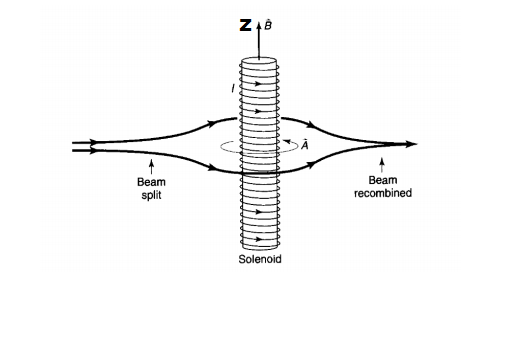
\includegraphics[scale=1]{img/solenoide.png}
\caption{Solenoide de longitud infinita con eje de simetría alineado con el eje z. El campo magnético $\vec{B}$ es homogéneo dentro del solenoide y esta alineado con el eje z, fuera del solenoide $\vec{B}$ es cero. Se demuestra que las ondas que generan el patrón de interferencia tienen un desfase adicional $\Delta \Phi =\frac{e}{\hbar}\Phi_m$ al esperado clásicamente, este desfase es consecuencia del flujo magnético en el solenoide (imagen tomada de \cite{1})}
\end{figure}

Si queremos resolver la ecuación de Shrodinger para una partícula cargada en la vecindad de este solenoide debemos encontrar primero una expresión para el potencial vectorial $\vec{A}$ y el potencial escalar $\phi$. Como el solenoide esta descargado, el campo eléctrico $\vec{E}=-\nabla\phi=0$, teniendo en cuenta que $\vec{B}$ no depende del tiempo, entonces $\frac{\partial \vec{A}}{\partial t}=0$ en consecuencia tenemos que $\phi$ es constante en el espacio y podemos escoger $\phi=0$. Como el campo magnético debe anularse fuera del solenoide $\vec{A}$ debe cumplir $\vec{B}=\nabla\times\vec{A}=0$. Por el teorema de Stokes sabemos que:


\begin{equation}
\oint_C \vec{A}\cdot \,d\vec{r}=\int_S (\nabla \times \vec{A}) \cdot \, d\vec{S}=\int_S\vec{B} \cdot \, d\vec{S}=\Phi_m 
\end{equation}


Donde $\Phi_m$ el el flujo total de campo magnético, y C es un camino circular cerrado de longitud $2\pi r$ alrededor del solenoide y que siempre es paralelo al vector $\vec{A}$ por lo que:

\begin{equation}
\oint_C \vec{A}\cdot \,d\vec{r}=|\vec{A}|2\pi r=\Phi_m
\end{equation}

donde $|\vec{A}|=A$ entonces 
\begin{equation}
\vec{A}=\frac{\Phi_m}{2\pi r}\hat{\phi}
\end{equation}


y $\hat{\phi}$ es el vector unitario en la dirección circular de las coordenadas cilíndricas y r es la distancia desde el eje z.

Para resolver la ecuación de Shrodinger definimos 


\begin{equation}
\Psi(\vec{r},t)=e^{ig(\vec{r})}\Psi'(\vec{r},t)
\end{equation}

\begin{equation}
g(\vec{r})=\frac{e}{\hbar}\int_{0}^{\vec{r}} \vec{A}(\vec{r})\cdot \,d\vec{r}
\end{equation}


Si sustituimos esta función de onda en la ecuación de Shrodinger nos va a quedar una ecuación como la siguiente:

\begin{equation}
-\frac{\hbar^2}{2m}\nabla^2\Psi'-V\Psi'=i\hbar\frac{\partial \Psi'}{\partial t}
\end{equation}


Advertimos de inmediato que esta es la ecuación de Shrodinger en ausencia de campo magnético, por lo cual podemos concluir que la función de onda asociada a una partícula cuántica en presencia de un campo magnético es la función de onda de la partícula cuando el campo esta ausente multiplicada por un factor de fase $e^{ig(\vec{r})}$

\section{Efecto Aharonov-Bohm}
Existen dos versiones del efecto AB: 
\begin{itemize}
\item Efecto AB eléctrico
\item efecto AB magnético
\end{itemize}

\subsection{Efecto AB Magnético}
Para demostrar experimentalmente el efecto AB magnético se realiza el siguiente experimento:

Supongamos dos haces de electrones que pasan a los lados de un solenoide tal como se observa en la figura 2. Se espera que, tal como en el experimento de difracción de doble rendija, se genere un patrón de interferencia entre los haces al llegar juntarse al otro lado del solenoide. Escribimos la función de onda de los haces en forma de ondas planas como sigue:


\begin{equation}
\Psi_1=Ae^{ikx_1}, \Psi_2=Ae^{ikx_2}
\end{equation}


donde k es el vector de onda de los electrones y $x_1$ y $x_2$ son las distancias recorridas por los haces.
En ausencia de campo electromagnético, el patrón de difracción dependerá únicamente de la distancia de caminos. Cuando se enciende un campo magnético, hemos visto que ocurre un desfase en las ondas que depende de $\vec{A}$, en consecuencia, existirá una diferencia de fase adicional dada por :

\begin{equation}
\Delta \Phi =g2-g1=\frac{e}{\hbar}[\oint_{C_2} \vec{A}\cdot \,d\vec{r}-\oint_{C_1} \vec{A}\cdot \,d\vec{r}]=\oint_{C} \vec{A}\cdot \,d\vec{r}=\frac{e}{\hbar}\Phi_m
\end{equation}
\begin{equation}
\boxed{\Delta \Phi =\frac{e}{\hbar}\Phi_m}
\end{equation}

De la ecuación anterior podemos concluir que el desfase entre haces es directamente proporcional al flujo magnético dentro del solenoide. Por lo que el patrón de interferencia se correrá. Este fenómeno es el llamado efecto de Aharonov-Bohm (efecto AB).
Observamos que una transformación de Gauge $A'=A+\nabla\chi$ no cambia el resultado anterior, ya que la integral cerrada sobre el gradiente de una función es cero. Por lo que el desfase es invariante bajo la transformación de Gauge.
 \cite{2}
\subsection{Efecto AB eléctrico}
En este enfoque del efecto las partículas pasan por una región donde el campo eléctrico es cero, pero el potencial $\phi$ no lo es. \\
Como sabemos la función de onda de una partícula cuántica evoluciona en el tiempo de la forma siguiente:
\begin{equation}
\Psi(\vec{r},t)=\Psi(\vec{r},t=0)e^{\frac{iEt}{\hbar}}
\end{equation}
vemos que (51) tiene la forma de (45) con $g=\frac{Et}{\hbar}$, sabemos que $E=e\phi$, por lo que podemos reescribir
\begin{equation}
g=\frac{e}{\hbar} \int_{0}^{t} \phi dt'
\end{equation}
Para que exista un desfase entre dos haces de partículas, estas deben pasar a través de regiones con potenciales $\phi$ distintos.
Entonces 

\begin{equation}
g_2-g_1= \frac{e}{\hbar}\int_{0}^{t} (\phi_2-\phi_1)dt'=\frac{e}{\hbar}\Delta \phi t 
\end{equation}
\begin{equation}
\boxed{\Delta \Phi = \frac{e}{\hbar}\Delta \phi t}
\end{equation}

\begin{figure}[H]
\centering
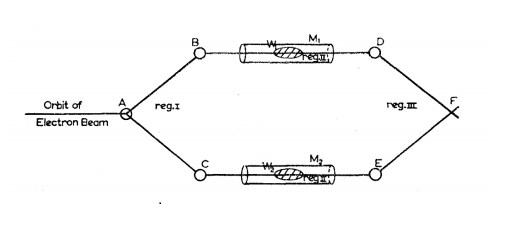
\includegraphics[scale=1]{img/electricAB.png}
\caption{Un haz de electrones es separado para hacerlo pasar por dos regiones con distinto potencial $\phi$, luego los haces vuelven a unirse para crear un patrón de interferencia}
\end{figure}

Donde $\Delta \phi$ es la diferencia de potencial entre los cilindros que aparecen en la figura 3. y t es el tiempo que tarda el haz de partículas en pasar a través del cilindro.
El resultado sera similar al del experimento anterior, se producirá un desfase en el patrón de interferencia 

\subsection{Efecto AB en superconductores}
Cuando están por debajo de una temperatura critica los superconductores no permiten la presencia de campos magnéticos en su interior, este fenomeno es llamado \textit{Efecto Meissner} 

\begin{figure}[H]
\centering
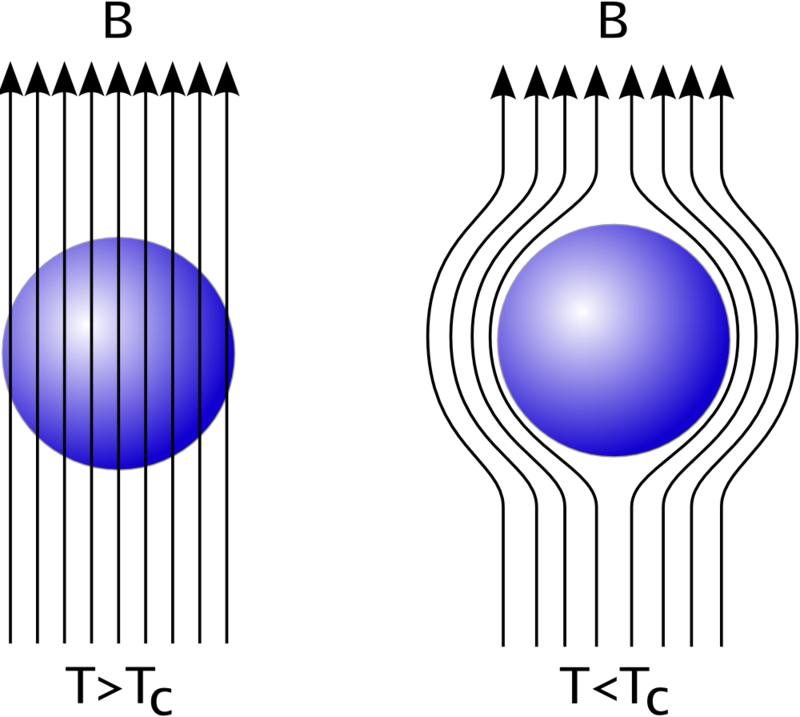
\includegraphics[scale=.3]{img/meisser.png}
\caption{Cuando el superconductor alcanza una temperatura critica muy baja $t_c$ este no permite el flujo de campo magnético en su interior. Este fenomeno se conoce como \textit{Efecto Meissner} }
\end{figure}

Pero en los superconductores de tipo 2, (que se diferencian de los de tipo 1 en que estos pasan al estado superconductor y no bruscamente como los de tipo 1) en la presencia de fuertes campos magnéticos pueden permitir el paso de lineas de campo magnético. Pero con la característica especial que estas lineas de campo estarán cuantizadas. Si imaginamos estas lineas de flujo magnético como pequeños solenoides, podemos hacer una analogía con el caso ya estudiado del efecto AB magnético.\\
En este caso queremos demostrar que el flujo estará cuantizado y es de la forma:
\begin{equation}
\Phi=\frac{nh}{2e_o}
\end{equation}
$e_o$ es la carga del electrón y n es un numero entero.
Si nos alrededor de una de estas lineas de flujo, como vimos anteriormente, esta presentara un desfase $e^{ig}$, para que la función sea monovaluada entonces $e^{ig}=1$, entonces
\begin{equation}
\cos(g)=1
\end{equation}
y por ecuación (45)
\begin{equation}
g=\frac{e\Phi_m}{\hbar}
\end{equation}

\begin{equation}
\implies \frac{e\Phi_m}{\hbar}=2\pi n
\end{equation}
\begin{equation}
\therefore \Phi_m=\frac{nh}{e}
\end{equation}
vemos que se obtiene el resultado correcto solo si hacemos $e=2e_o$, este resultado nos indica que dentro del superconductor hay un tipo de partícula llamada \textit{Pares de Cooper}, la cual esta formada por dos electrones que se atraen (aunque parezca increíble, ya que ambos poseen igual carga). La formación de los pares de Cooper se debe a la interacción de los electrones con la red cristalina que forma el superconductor.


\bibliographystyle{alpha}
\bibliography{sample}

\end{document}